\chapter[Figuras Adicionais]{Figuras Adicionais}
\label{ape:figuras}

As figuras a seguir complementam as análises do Capítulo~\ref{experimentos}.

\section{Curvas de Convergências}

As \autoref{fig:ape-conv-10a} a \autoref{fig:ape-conv-100a} apresentam as curvas de convergência para instâncias representativas. Cada gráfico mostra a evolução do makespan da melhor solução ao longo das iterações para GA, PSO e ACO.

\begin{figure}[htbp]
\centering
\caption{Convergência na instância 10a.}
\label{fig:ape-conv-10a}
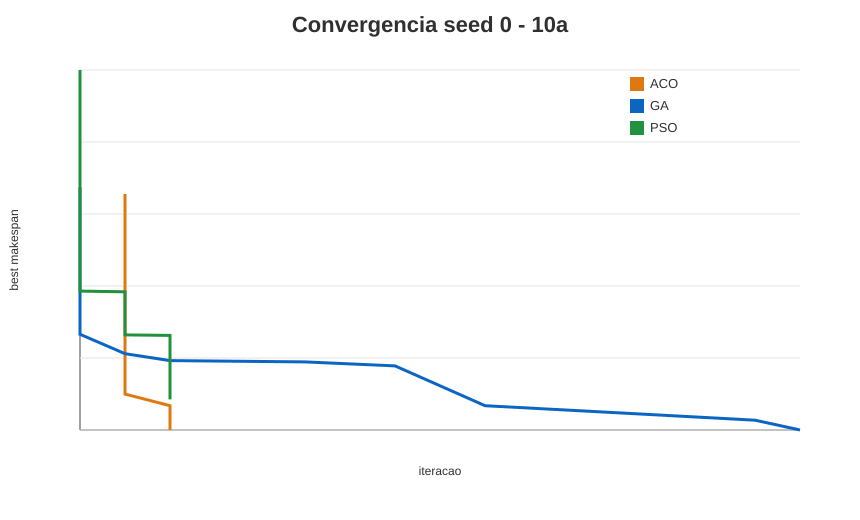
\includegraphics[width=\textwidth]{figs/convergence-overlay-10a.png}
\legend{Fonte: dados da pesquisa.}
\end{figure}

\begin{figure}[htbp]
\centering
\caption{Convergência na instância 30a.}
\label{fig:ape-conv-30a}
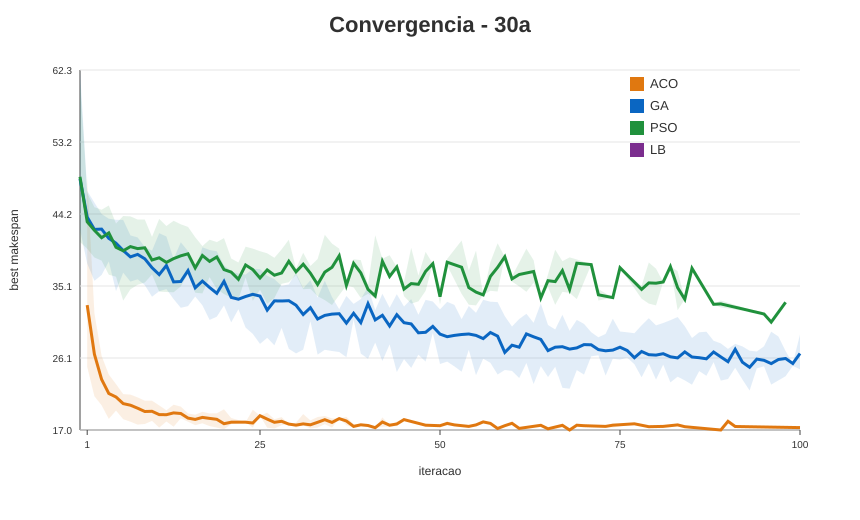
\includegraphics[width=\textwidth]{figs/convergence-overlay-30a.png}
\legend{Fonte: dados da pesquisa.}
\end{figure}

\begin{figure}[htbp]
\centering
\caption{Convergência na instância 50a.}
\label{fig:ape-conv-50a}
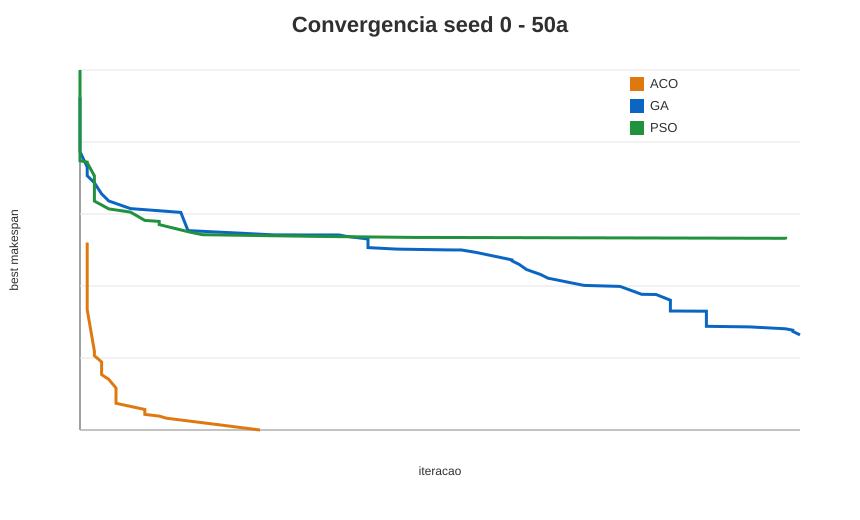
\includegraphics[width=\textwidth]{figs/convergence-overlay-50a.png}
\legend{Fonte: dados da pesquisa.}
\end{figure}

\begin{figure}[htbp]
\centering
\caption{Convergência na instância 100a.}
\label{fig:ape-conv-100a}
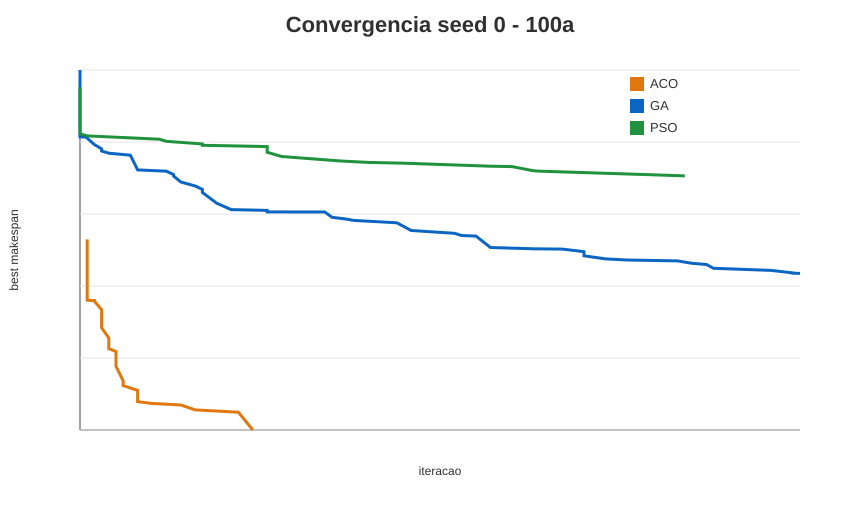
\includegraphics[width=\textwidth]{figs/convergence-overlay-100a.png}
\legend{Fonte: dados da pesquisa.}
\end{figure}

\section{Painéis de Rotas}

As \autoref{fig:ape-route-10a} a \autoref{fig:ape-route-100a} apresentam as rotas obtidas por cada método em instâncias representativas.

\begin{figure}[htbp]
\centering
\caption{Comparação de rotas na instância 10a.}
\label{fig:ape-route-10a}
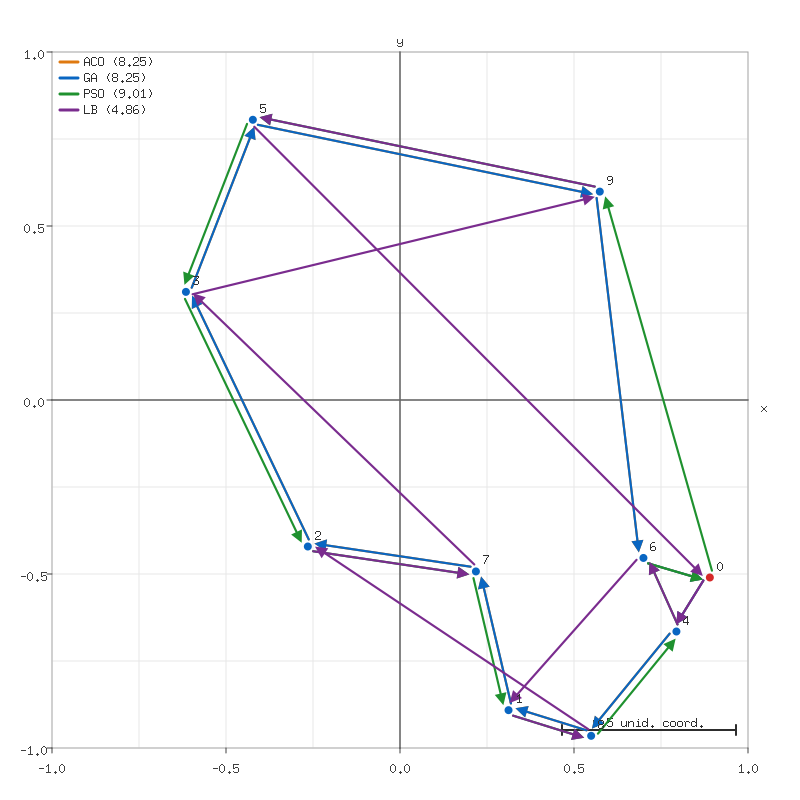
\includegraphics[width=\textwidth]{figs/route-panel-10a.png}
\legend{Fonte: dados da pesquisa.}
\end{figure}

\begin{figure}[htbp]
\centering
\caption{Comparação de rotas na instância 30a.}
\label{fig:ape-route-30a}
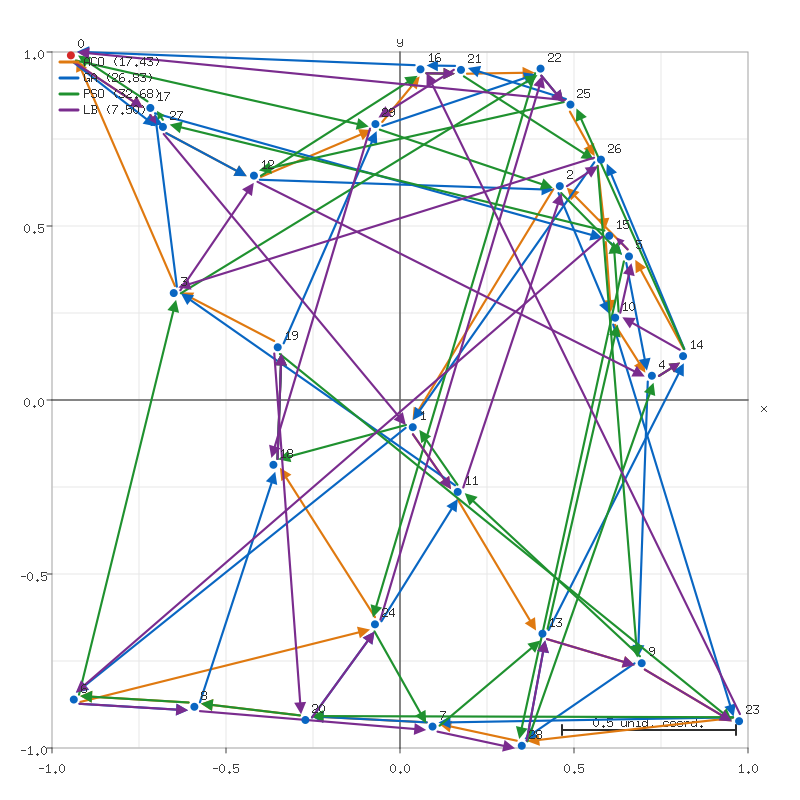
\includegraphics[width=\textwidth]{figs/route-panel-30a.png}
\legend{Fonte: dados da pesquisa.}
\end{figure}

\begin{figure}[htbp]
\centering
\caption{Comparação de rotas na instância 100a.}
\label{fig:ape-route-100a}
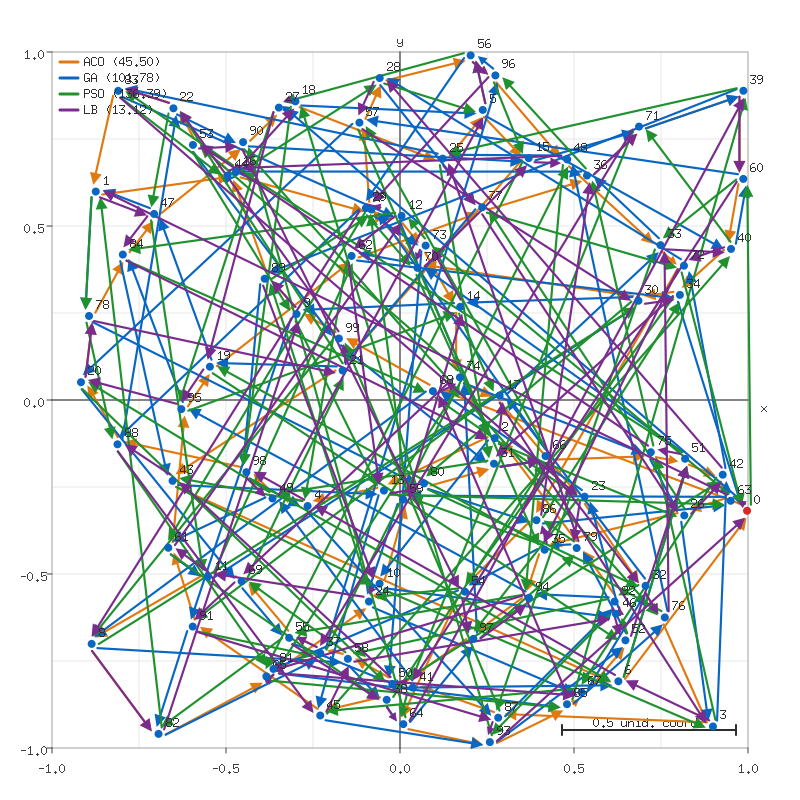
\includegraphics[width=\textwidth]{figs/route-panel-100a.png}
\legend{Fonte: dados da pesquisa.}
\end{figure}

\section{Estabilidade entre Sementes}

A \autoref{fig:ape-estabilidade} apresenta a distribuição dos makespans obtidos pelas 51 sementes de cada método, agregados por instância.

\begin{figure}[htbp]
\centering
\caption{Estabilidade dos métodos entre sementes.}
\label{fig:ape-estabilidade}
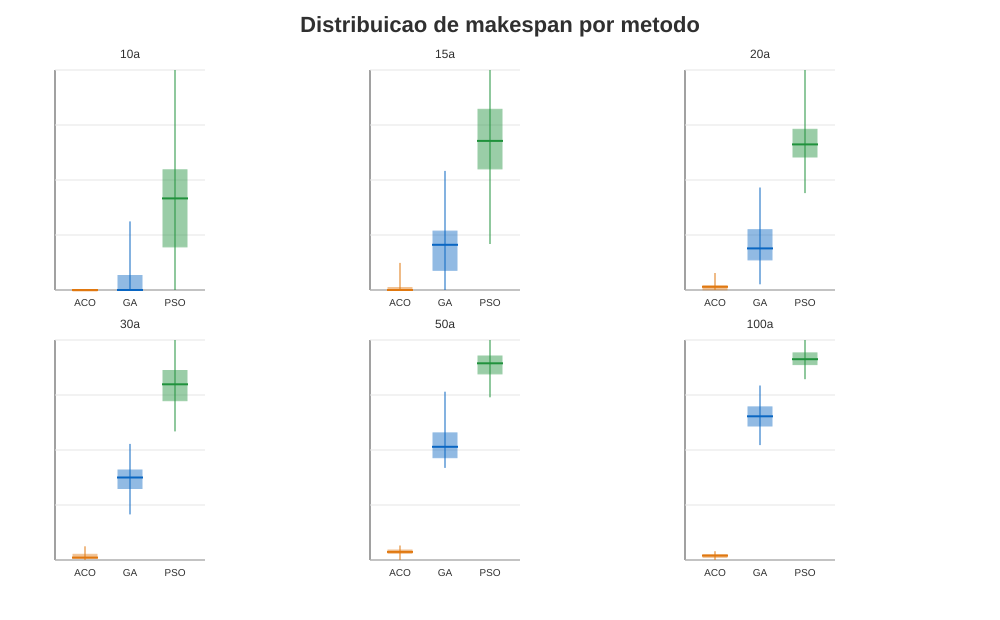
\includegraphics[width=\textwidth]{figs/boxplot-estabilidade.png}
\legend{Fonte: dados da pesquisa.}
\end{figure}
